\documentclass[12pt,aspectratio=169,t]{beamer}
\usetheme{windclim}
\graphicspath{{figures/}{./}}

\title{JRA-3Qを用いた\\高層風の\\統計的傾向の解析}
\author{西濱大将}
\date{}

% Sources cited on the slides as (Key+YY). Full entries are in references.md.
\defref{Kosaka+24}{Kosaka, Y. et al. (2024). The JRA-3Q Reanalysis. \emph{J. Meteor. Soc. Japan}, 102, 49--109. doi:10.2151/jmsj.2024-004}
\defref{JMA+24}{Japan Meteorological Agency (2024). JRA-3Q. NSF NCAR GDEX, dataset d640000. CC BY-NC-SA 4.0}
\defref{Hersbach+20}{Hersbach, H. et al. (2020). The ERA5 global reanalysis. \emph{Q. J. R. Meteorol. Soc.}, 146, 1999--2049. doi:10.1002/qj.3803}
\defref{Gelaro+17}{Gelaro, R. et al. (2017). MERRA-2. \emph{J. Climate}, 30, 5419--5454. doi:10.1175/JCLI-D-16-0758.1}
\defref{Kobayashi+15}{Kobayashi, S. et al. (2015). The JRA-55 Reanalysis. \emph{J. Meteor. Soc. Japan}, 93, 5--48. doi:10.2151/jmsj.2015-001}
\defref{Kalnay+96}{Kalnay, E. et al. (1996). The NCEP/NCAR 40-Year Reanalysis Project. \emph{Bull. Amer. Meteor. Soc.}, 77, 437--471}
\defref{Wilks+11}{Wilks, D. S. (2011). \emph{Statistical Methods in the Atmospheric Sciences}, 3rd ed. Academic Press}
\defref{Mardia+00}{Mardia, K. V., Jupp, P. E. (2000). \emph{Directional Statistics}. Wiley}
\defref{Hastie+09}{Hastie, T., Tibshirani, R., Friedman, J. (2009). \emph{The Elements of Statistical Learning}, 2nd ed. Springer}
\defref{Harvey+96}{Harvey, V. L., Hitchman, M. H. (1996). A Climatology of the Aleutian High. \emph{J. Atmos. Sci.}, 53, 2088--2101}
\defref{Baldwin+01}{Baldwin, M. P. et al. (2001). The quasi-biennial oscillation. \emph{Rev. Geophys.}, 39, 179--229. doi:10.1029/1999RG000073}
\defref{ICAO+93}{ICAO (1993). \emph{Manual of the ICAO Standard Atmosphere}, Doc 7488/3}


\begin{document}
\titleframe
\begin{frame}{JRA-3Qとは？}{データ}
  \lead{気象庁の第 3 次長期再解析。$u, v, Z$ を 10 年ぶん使う \src{Kosaka+24}}
  \begin{cards}[3]
    \minicard{th-large}{0.375°}{約 40 km 格子}
    \minicard{layer-group}{38 面}{1000--3 hPa、約 0--40 km}
    \minicard{clock}{6 時間 × 10 年}{2016--2025、14,610 時刻}
  \end{cards}
  \vskip 1.5mm
  \begin{columns}[T]
    \begin{column}{0.72\textwidth}
      \begin{itemize}\itemsep 0.2mm
        \item \kw{なぜ JRA-3Q か}：国内の観測を厚く同化した気象庁製品
        \item 上端 0.01 hPa（約 80 km）。破裂高度を余裕で覆う
        \item 1947 年から現在まで。GDEX から無償 \src{JMA+24}
      \end{itemize}
    \end{column}
    \begin{column}{0.24\textwidth}
      \vskip -3mm
      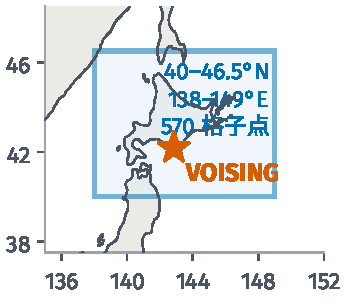
\includegraphics[width=\linewidth,height=70pt,keepaspectratio]{S_region_map.pdf}
    \end{column}
  \end{columns}
  \srcline{領域は北海道の箱 570 格子点、代表地点は VOISING。和歌山は比較用}
\end{frame}

\begin{frame}{JRA-3Qとは？}{データ}
  \lead{高さも細かさも足りる再解析は 3 つ。本研究は JRA-3Q}
  {\centering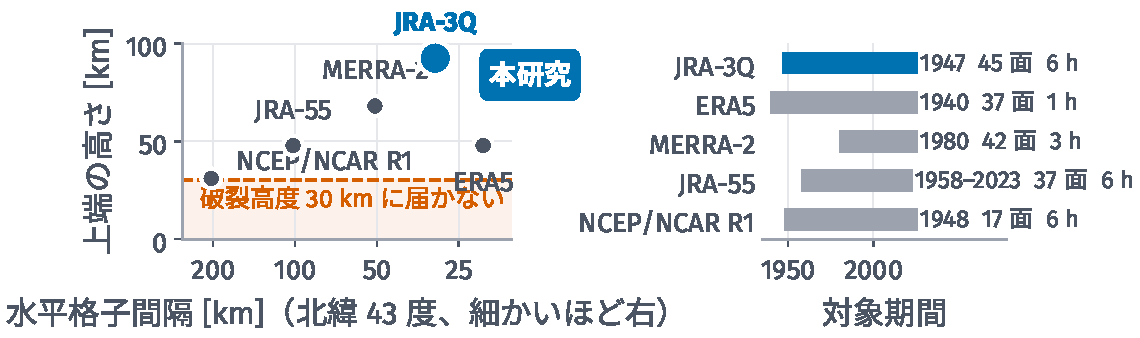
\includegraphics[width=0.92\linewidth,height=104pt,keepaspectratio]{S_reanalyses.pdf}\par}
  \vskip 1mm
  \sub{格子間隔は北緯 43 度での値。JRA-3Q は実測、他は各機関の公表仕様。}
  \srcline{\src{Kalnay+96} \src{Kobayashi+15} \src{Gelaro+17} \src{Hersbach+20}}
\end{frame}

\begin{frame}{データセットの下準備}{手法：時間の切り方}
  \lead{時間は「半月」で切る。データが支える最も細かい単位は 15 日}
  \begin{columns}[T]
    \begin{column}{0.40\textwidth}
      \begin{center}
      \begin{tikzpicture}[x=1mm,y=1mm]
        \fill[wcPale] (0,0) rectangle (25,6.5);
        \fill[wcBlue!25] (25,0) rectangle (50,6.5);
        \draw[wcMuted,line width=0.5pt] (0,0) rectangle (50,6.5);
        \draw[wcBlue,line width=0.9pt] (25,0) -- (25,6.5);
        \node[font=\mediumfont\fontsize{10}{12}\selectfont,text=wcText] at (12.5,3.25) {前半 1--15 日};
        \node[font=\mediumfont\fontsize{10}{12}\selectfont,text=wcText] at (37.5,3.25) {後半 16 日--月末};
      \end{tikzpicture}
      \end{center}
      \vskip 0.5mm
      \sub{1 年抜きの交差検証（10 通り）}
      \vskip -1.5mm
      \[
        \text{誤差の削減} = 1 - \frac{\mathrm{RMSE}}{\mathrm{RMSE}_{\text{季節なし}}}
      \]
      \vskip -3mm
      \sub{2 SE 以内は区別できない \src{Hastie+09}}
    \end{column}
    \begin{column}{0.58\textwidth}
      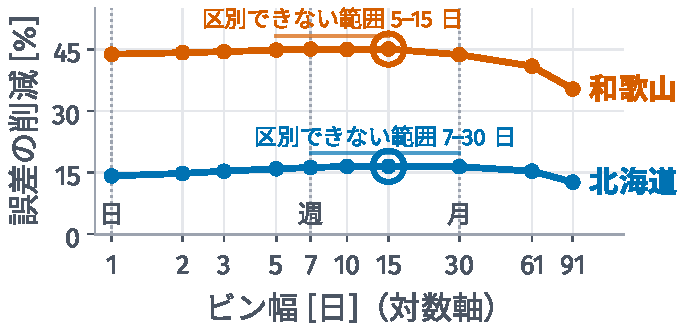
\includegraphics[width=\linewidth,height=136pt,keepaspectratio]{S_skill_overlay.pdf}
    \end{column}
  \end{columns}
  \srcline{年 24 ビン、各 520--640 解析値。落下位置のベクトル RMSE、2016--2025}
\end{frame}

\begin{frame}{データセットの下準備}{手法：平均風速と平均風向}
  \lead{風向は平均しない。$u, v$ を平均してから向きに戻す}
  \begin{columns}[T]
    \begin{column}{0.36\textwidth}
      \begin{center}
      \begin{tikzpicture}[x=1mm,y=1mm,>={Latex[length=2.2mm,width=1.8mm]}]
        \draw[wcMuted,line width=0.5pt] (0,0) circle (10);
        \draw[wcMuted,line width=0.5pt] (0,-11.5) -- (0,11.5);
        \draw[wcMuted,line width=0.5pt] (-11.5,0) -- (11.5,0);
        \node[font=\fontsize{8.5}{10}\selectfont,text=wcSecondary] at (0,13.5) {北};
        \draw[->,wcBlue,line width=1.3pt] (0,0) -- (-1.2,9.6);
        \draw[->,wcBlue,line width=1.3pt] (0,0) -- (1.2,9.6);
        \node[font=\fontsize{9}{10}\selectfont,text=wcBlue,anchor=east] at (-2,8.5) {359°};
        \node[font=\fontsize{9}{10}\selectfont,text=wcBlue,anchor=west] at (2,8.5) {1°};
        \draw[->,wcOrange,line width=1.3pt,dashed] (0,0) -- (0,-9.6);
        \node[font=\mediumfont\fontsize{9.5}{11}\selectfont,text=wcOrange,anchor=north] at (0,-12) {算術平均 180°（南）×};
        \draw[->,wcBlue,line width=1.8pt] (24,0) -- (24,9.6);
        \node[font=\mediumfont\fontsize{9.5}{11}\selectfont,text=wcBlue,anchor=north,align=center] at (24,-1.5) {ベクトル平均\\0°（北）○};
      \end{tikzpicture}
      \end{center}
      \vskip 0.5mm
      \sub{算術平均だと北風 2 回が南風に}
    \end{column}
    \begin{column}{0.62\textwidth}
      \vskip -5mm
      {\small
      \begin{align*}
        \bar u &= \tfrac{1}{N}\textstyle\sum_i u_i, \qquad \bar v = \tfrac{1}{N}\textstyle\sum_i v_i \\[-0.5mm]
        \theta &= \bigl(\operatorname{atan2}(\bar u, \bar v)\,\tfrac{180}{\pi} + 180\bigr) \bmod 360 \\[1mm]
        \text{ベクトル平均}\quad \lvert\bar{\mathbf V}\rvert &= \sqrt{\bar u^2 + \bar v^2} \\[-0.5mm]
        \text{スカラー平均}\quad \overline{\lvert\mathbf V\rvert} &= \tfrac{1}{N}\textstyle\sum_i \sqrt{u_i^2 + v_i^2} \\[1mm]
        \text{定常度}\quad C &= \lvert\bar{\mathbf V}\rvert \big/ \overline{\lvert\mathbf V\rvert} \in [0, 1]
      \end{align*}}
      \vskip -3mm
      \sub{\kw{$C < 0.3$} の風向は図で灰色にする\\\src{Mardia+00}}
    \end{column}
  \end{columns}
  \srcline{ベクトル平均は正味の移動、スカラー平均は強さ。風向は吹いてくる向き}
\end{frame}

\begin{frame}{意味のある「統計」期間について}{検証}
  \lead{実在するのは 1〜2 か月スケールの季節変化}
  \begin{columns}[T]
    \begin{column}{0.44\textwidth}
      \sub{1 年を $K$ 個の正弦波で表す（調和回帰）}
      \vskip -4mm
      {\small
      \begin{align*}
        \hat{\mathbf y}(d) = \mathbf a_0 + \sum_{j=1}^{K}\Bigl[&\mathbf a_j \cos\bigl(\tfrac{2\pi j d}{365}\bigr) \\[-1mm]
          &+ \mathbf b_j \sin\bigl(\tfrac{2\pi j d}{365}\bigr)\Bigr]
      \end{align*}}
      \vskip -3.5mm
      \begin{itemize}\itemsep 0.3mm
        \item 分解能 $\tau(K) = 365 / (2K)$ 日
        \item 誤差は \kw{$K = 5$--$6$} で頭打ち：$\tau \approx 30$--$36$ 日
        \item 半月ビンはこれを表現する単位
      \end{itemize}
    \end{column}
    \begin{column}{0.54\textwidth}
      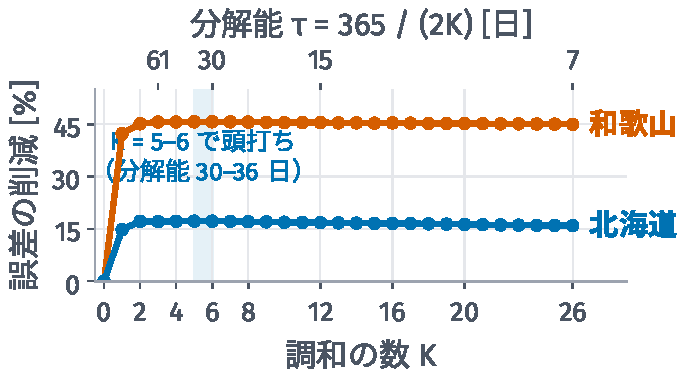
\includegraphics[width=\linewidth,height=124pt,keepaspectratio]{S_harmonic_overlay.pdf}
    \end{column}
  \end{columns}
  \srcline{1 年抜き交差検証、落下位置のベクトル RMSE}
\end{frame}

\begin{frame}{意味のある「統計」期間について}{検証}
  \lead{上空の対流圏の風は、時期を知ってもほとんど当てられない}
  \begin{columns}[T]
    \begin{column}{0.56\textwidth}
      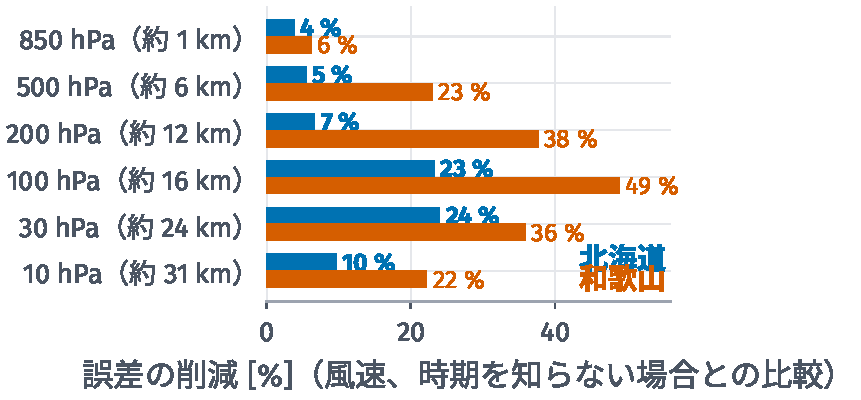
\includegraphics[width=\linewidth,height=126pt,keepaspectratio]{S_level_skill_both.pdf}
    \end{column}
    \begin{column}{0.42\textwidth}
      \begin{itemize}\itemsep 1.5mm
        \item \kw{地上付近は 4--6 \%}\\地上風は当日の予報で判断する
        \item \kw{北海道の 200 hPa は 7 \%}\\ジェットの高さでも暦は効かない
        \item 役に立つのは \kw{16--24 km}\\（100--30 hPa の帯）
      \end{itemize}
    \end{column}
  \end{columns}
  \srcline{風速の 1 年抜き交差検証、最良ビン幅でのスキル}
\end{frame}

\begin{frame}{秋にジェットが最も強く、\\対流圏の風向は年中読みやすい}{結果：北海道}
  \begin{columns}[T]
    \begin{column}{0.62\textwidth}
      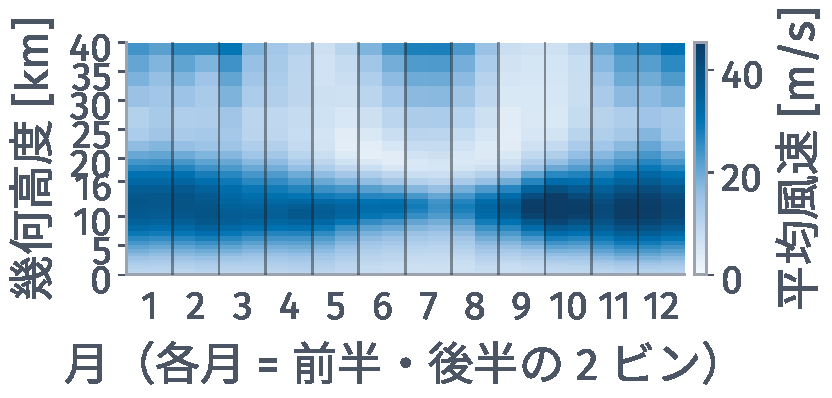
\includegraphics[width=\linewidth,height=96pt,keepaspectratio]{S_alt_half_speed.pdf}
      \vskip 0.5mm
      \sub{ジェットは冬に最強で、同時に南へ下がる。\\北海道には \kw{10--11 月に核が通過}する。}
    \end{column}
    \begin{column}{0.30\textwidth}
      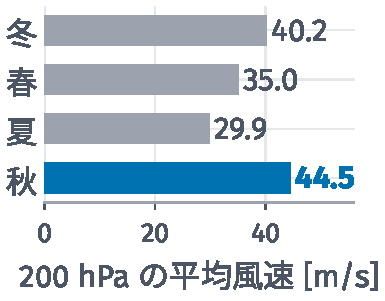
\includegraphics[width=\linewidth,height=88pt,keepaspectratio]{S_season_speed_200.pdf}
      \vskip 0.5mm
      \sub{定常度 \kw{0.81--0.96}、\\風向は年中信用できる。}
    \end{column}
  \end{columns}
  \srcline{北海道 570 格子点の領域平均、2016--2025。和歌山の最強は冬（75.5 m/s）}
\end{frame}

\begin{frame}{破裂高度帯は春と秋に風向が読めない}{結果：北海道}
  \begin{columns}[T]
    \begin{column}{0.56\textwidth}
      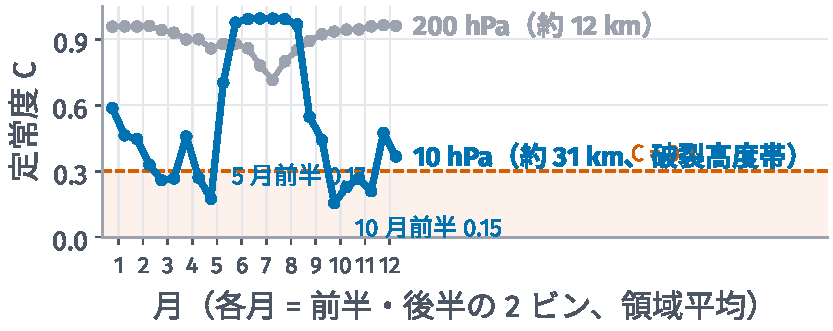
\includegraphics[width=\linewidth,height=118pt,keepaspectratio]{S_constancy_10hpa.pdf}
      \vskip 0.5mm
      \sub{夏 0.99、春 0.35、秋 0.31。東西逆転の時期は\\\kw{西風の日}と\kw{東風の日}が混ざり、打ち消し合う。}
    \end{column}
    \begin{column}{0.42\textwidth}
      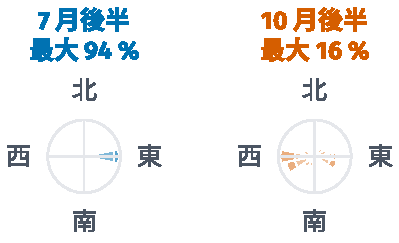
\includegraphics[width=\linewidth,height=96pt,keepaspectratio]{S_roses_10hpa.pdf}
      \vskip 0.5mm
      \sub{\warn{データが無いのではない}。\\平均風向に意味がない。}
    \end{column}
  \end{columns}
  \srcline{10 hPa（約 31 km）。定常度は領域平均、風配図は 1 格子点（半径は図ごと）}
\end{frame}

\begin{frame}{冬の 10 hPa が東風なのは\\アリューシャン高気圧の西縁だから}{考察}
  \begin{columns}[T]
    \begin{column}{0.44\textwidth}
      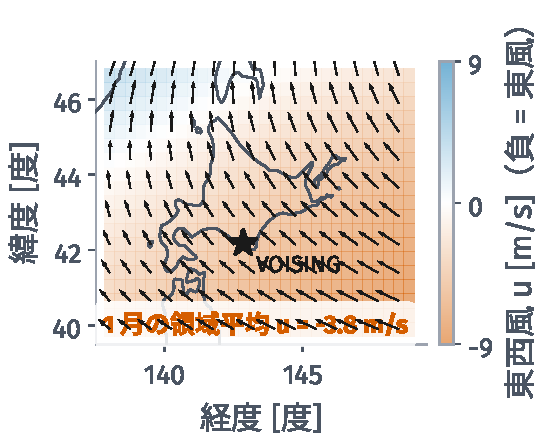
\includegraphics[width=\linewidth,height=124pt,keepaspectratio]{S_map_10hpa_jan.pdf}
    \end{column}
    \begin{column}{0.54\textwidth}
      {\centering
      \begin{tikzpicture}[x=1mm,y=1mm,>={Latex[length=2mm,width=1.6mm]}]
        \fill[wcGrey] (-33,-9) rectangle (33,9);
        \node[font=\fontsize{8.5}{10}\selectfont,text=wcSecondary,anchor=north west] at (-32.5,8.5) {北太平洋の成層圏（10 hPa、真冬）};
        \draw[wcBlue,line width=1.2pt,->] (15,-2.5) ++(150:10 and 4.8) arc (150:-160:10 and 4.8);
        \node[font=\mediumfont\fontsize{8.5}{10}\selectfont,text=wcBlue,align=center] at (15,-2.5) {アリューシャン\\高気圧};
        \fill[wcMuted] (-19,-3.5) ellipse (2 and 3.6);
        \node[font=\fontsize{8.5}{10}\selectfont,text=wcSecondary,anchor=east] at (-21.5,-3.5) {日本};
        \draw[wcOrange,line width=1.5pt,->] (-4,-2.5) -- (-15,-2.5);
        \node[font=\mediumfont\fontsize{9}{10.5}\selectfont,text=wcOrange,anchor=north] at (-9.5,-3.6) {東風};
      \end{tikzpicture}\par}
      \vskip 0.8mm
      \begin{itemize}\itemsep 0.4mm
        \item 帯状平均では冬の中緯度成層圏は\kw{西風}
        \item 1 月の 10 hPa は\warn{東風 $-3.8$ m/s}、各年とも
        \item 高気圧の西縁にあたる \src{Harvey+96}
        \item 帯状平均を扇形の領域に当てはめない
      \end{itemize}
    \end{column}
  \end{columns}
\end{frame}

\begin{frame}{飛行距離は季節で 3.5 倍変わる}{結果：北海道の落下位置}
  \begin{columns}[T]
    \begin{column}{0.34\textwidth}
      \begin{center}
      \begin{tikzpicture}[x=1mm,y=1mm,>={Latex[length=2mm,width=1.6mm]}]
        \draw[wcMuted,line width=0.6pt] (0,0) -- (44,0);
        \draw[wcMuted,line width=0.5pt,dotted] (0,5) -- (44,5);
        \draw[wcMuted,line width=0.5pt,dotted] (0,10) -- (44,10);
        \node[font=\fontsize{8}{9}\selectfont,text=wcMuted,anchor=east] at (43.5,7.5) {層 $k$};
        \draw[wcBlue,line width=1.6pt,->] (2,0) -- (14,15);
        \node[font=\fontsize{8.5}{9.5}\selectfont,text=wcBlue,anchor=east,align=right] at (7.5,8.5) {上昇\\5 m/s};
        \fill[wcOrange] (14,15) circle (1.2);
        \node[font=\mediumfont\fontsize{8.5}{10}\selectfont,text=wcOrange,anchor=south] at (14,16.2) {破裂 30 km};
        \draw[wcBlue,line width=1.6pt,dashed,->] (14,15) -- (34,0);
        \node[font=\fontsize{8.5}{9.5}\selectfont,text=wcBlue,anchor=west,align=left] at (25,8.5) {降下\\6 m/s};
        \draw[wcSecondary,line width=0.7pt,<->] (2,-2.5) -- (34,-2.5);
        \node[font=\fontsize{8.5}{9.5}\selectfont,text=wcSecondary,anchor=north] at (18,-3) {$\Delta x$、約 137 分};
      \end{tikzpicture}
      \end{center}
      \vskip 0.5mm
      \sub{$\Delta x = \sum_k u_k T_k$\\$T_k$ は層 $k$ の滞在時間}
    \end{column}
    \begin{column}{0.64\textwidth}
      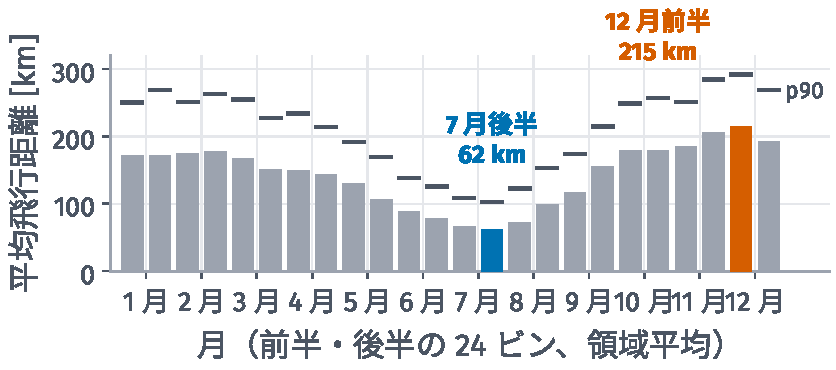
\includegraphics[width=\linewidth,height=108pt,keepaspectratio]{S_drift_by_bin.pdf}
      \vskip 0.5mm
      \sub{領域平均、進行方位は東北東でほぼ一定。\\11--12 月は平均 200 km 超、p90 は 300 km。}
    \end{column}
  \end{columns}
  \srcline{飛行モデルは既存シミュレータと同一。$T_k$ は風によらない}
\end{frame}

\begin{frame}{VOISING からの落下点は通年で海上}{結果：北海道の落下位置}
  \begin{columns}[T]
    \begin{column}{0.38\textwidth}
      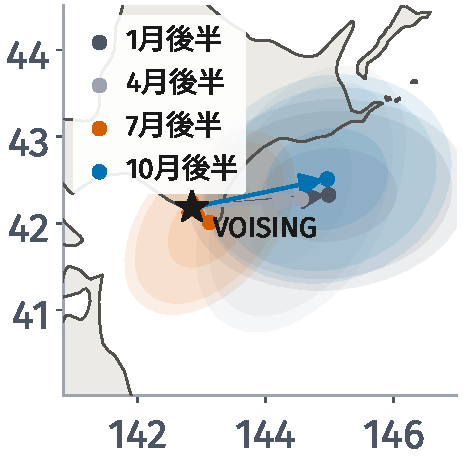
\includegraphics[width=\linewidth,height=140pt,keepaspectratio]{S_voising_landing_seasons.pdf}
    \end{column}
    \begin{column}{0.60\textwidth}
      \begin{columns}[T]
        \begin{column}{0.56\textwidth}
          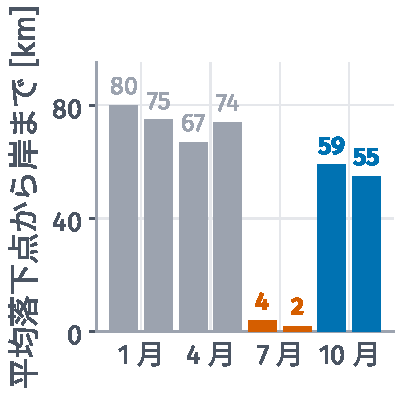
\includegraphics[width=\linewidth,height=100pt,keepaspectratio]{S_offshore_bars.pdf}
        \end{column}
        \begin{column}{0.42\textwidth}
          \vskip 1mm
          \midnum[wcOrange]{2--4}{km}{7 月だけ岸のすぐそば}
          \vskip 3mm
          \midnum{55--80}{km}{他の季節は沖。船が要る}
        \end{column}
      \end{columns}
      \vskip 1mm
      \sub{変わるのは「海か陸か」ではなく\kw{岸からの距離}。\\地点の性質。内陸から上げれば陸に落ちる。}
    \end{column}
  \end{columns}
  \srcline{楕円は 50 / 90 / 95 \%、各月の後半ビン。地点固有の結果、道北・道東には使わない}
\end{frame}

\begin{frame}{10 月下旬に VOISING から上げると\\東北東へ 185 km、岸から 55 km 沖}{予想}
  \begin{columns}[T]
    \begin{column}{0.38\textwidth}
      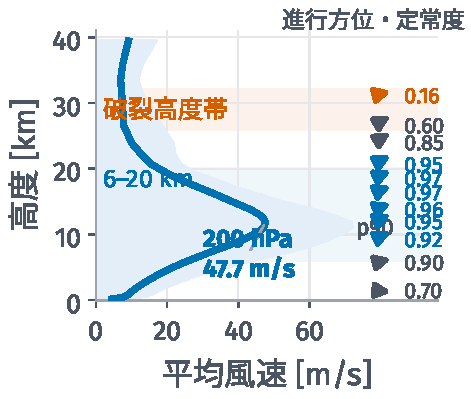
\includegraphics[width=\linewidth,height=130pt,keepaspectratio]{S_oct_profile.pdf}
    \end{column}
    \begin{column}{0.60\textwidth}
      \begin{columns}[T]
        \begin{column}{0.46\textwidth}
          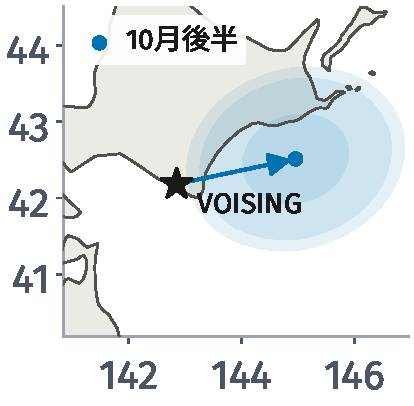
\includegraphics[width=\linewidth,height=90pt,keepaspectratio]{S_voising_landing_oct.pdf}
        \end{column}
        \begin{column}{0.52\textwidth}
          \midnum{185}{km}{平均飛行距離、進行方位 78°}
          \vskip 2mm
          \midnum{55}{km}{平均落下点から岸まで}
        \end{column}
      \end{columns}
      \vskip 1mm
      \sub{6--20 km は定常度 0.92--0.97 で向きは確か。\\20--10 hPa は 0.6 → 0.16 で向きが読めない。\\p90 は 257 km。\warn{1 日ずれると 56 km} 動く。}
    \end{column}
  \end{columns}
  \srcline{10 月後半ビン、VOISING 最寄り格子、2016--2025。予報誤差は含まない}
\end{frame}

\begin{frame}{北海道は読みにくい：\\暦で減らせる誤差は 17 \%}{考察}
  \begin{columns}[T]
    \begin{column}{0.34\textwidth}
      \bignum{17}{\%}{北海道：時期を知って減る\\落下位置の誤差}
      \vskip 3mm
      \midnum[wcOrange]{45}{\%}{和歌山（分散では 31 対 70 \%）}
    \end{column}
    \begin{column}{0.64\textwidth}
      {\centering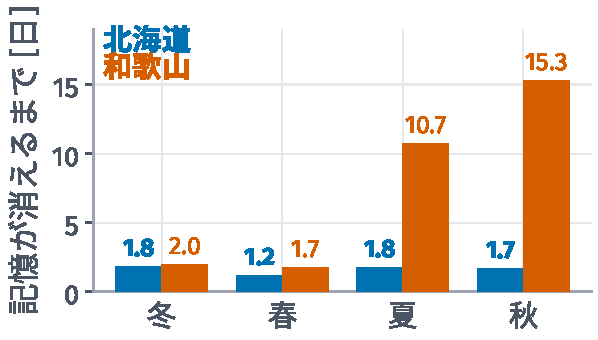
\includegraphics[width=0.86\linewidth,height=84pt,keepaspectratio]{S_decorrelation_200.pdf}\par}
      \vskip 0.5mm
      \sub{和歌山は夏・秋に 10--15 日、北海道は\kw{2 日}で入れ替わる。\\流れが止まらないので、記憶も伸びない。}
    \end{column}
  \end{columns}
  \srcline{200 hPa。風の偏差の自己相関が 1/e を切るまでの時間、2016--2025}
\end{frame}

\begin{frame}{効くのは日程のずれ：\\1 日で落下点が 43--63 km 動く}{考察}
  \begin{columns}[T]
    \begin{column}{0.58\textwidth}
      {\centering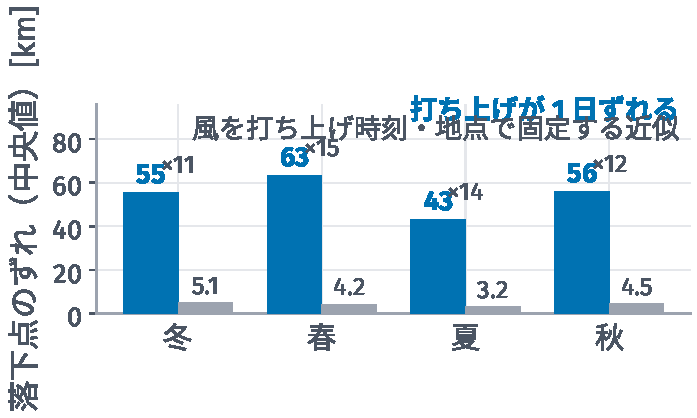
\includegraphics[width=\linewidth,height=100pt,keepaspectratio]{S_slip_vs_frozen.pdf}\par}
      \vskip 0.8mm
      \sub{風を固定する近似の誤差は 3--5 km。\\日程のずれより \kw{1 桁小さく}、直す価値は薄い。}
    \end{column}
    \begin{column}{0.40\textwidth}
      \begin{itemize}\itemsep 1.2mm
        \item \kw{夏}：ずれ 43 km で最小
        \item \kw{秋}：相対誤差 2.9 \% で最小
        \item \warn{春}：ずれ 63 km。避ける
      \end{itemize}
      \vskip 1.5mm
      \sub{すべて「予報が完璧なら」の話。\\予報誤差が上乗せされる。}
    \end{column}
  \end{columns}
  \srcline{北海道、格子の中を実際に飛ばした基準軌道との差（中央値）、2016--2025}
\end{frame}

\begin{frame}{この統計が言えないこと}{限界}
  \begin{cards}[4]
    \card[wcOrange]{cloud}{予報誤差}{測っていない。誤差は下限。}
    \card{history}{10 年}{QBO で 4--5 周期。10 年の癖が残る \src{Baldwin+01}}
    \card{mountain}{40 km}{日高山脈は 2--3 点。地形風は含まない。}
    \card{layer-group}{気圧面}{気圧面の高度は数百 m 動く。}
  \end{cards}
  \vskip 3mm
  \sub{再解析は観測ではない。25--35 km は観測が薄く、モデルの寄与が大きい。\\半月の平均は「その日」を教えない。飛ばす日の判断には予報を使う。}
\end{frame}

\begin{frame}{まとめ}{}
  \begin{cards}[2]
    \palecard{北海道の高層風の姿を捉えた}{秋にジェット最強。対流圏の風向は年中読め、破裂高度帯は春秋に読めない。}
    \palecard{意味のある統計期間は 1〜2 か月}{最細は 15 日。上空の対流圏は暦で当たらない（落下位置で 17 \%）。}
    \palecard{VOISING からは通年で海上}{10 月下旬は東北東へ 185 km、岸から 55 km。1 日ずれで 56 km 動く。}
    \palecard[wcOrange]{気候値は計画の道具}{風の固定の近似は 3--5 km で、日程のずれの 1 桁下。当日の判断は予報で。}
  \end{cards}
\end{frame}

\begin{frame}[plain]{}
  \vskip 5mm
  {\heavyfont\fontsize{13}{16}\selectfont\color{wcText}参考文献\par}
  \vskip 2mm
  \printrefs
  \vskip 1mm
  {\fontsize{8.5}{10.5}\selectfont\color{wcSecondary}データ：JRA-3Q（気象庁）、NSF NCAR GDEX d640000、CC BY-NC-SA 4.0\par}
\end{frame}

\end{document}
